\section{Neural Network Modeling}
\label{NN}

The CHP plant described in previous Section has been modeled by means of several interconnected NNs as it is showed in Figure \ref{fignns}. Each NN handles one of the main components of the plant above mentioned. Thus, there are a total of 12 NNs: 4 for the engines, 4 for the engine cooling  circuits, one for the exhaust steam boiler, one for the steam turbine condenser, one for the steam turbine and finally another one for the slurry drying process. All the NNs are actually Multilayer Perceptrons with just one hidden layer. In all of them, the number of neurons of the hidden layer is twice the number of inputs and there is only one neuron in the output layer (i.e., each NN computes just a single output value). These outputs are respectively: a) the temperature of the water to cooling each engine ($T_{Mixt\_EngA}, \dots, T_{Mixt\_EngD}$; b) The flow of fuel (i.e. natural gas) required by each engine ($F_{Gas_A} \dots F_{Gas_D}$); c) The pressure of the condenser ($P_{CON}$); d) the steam flow in the boiler ($F_{Steam}$); e) the electric power produced by the turbine ($POW_{ST}$) and f) the flow of slurry processed by the evaporator ($F_{EV}$). 

To train and test the NNs a big data set was collected trough a one-year lecture process in the real plant. A total of  213 variables where acquired every minute during that period. First, a careful analysis of the data was performed to chose the most relevant variables and also to filter outliers, missing data or un-informative variables. %Input variables in the models were selected by the authors, based on the knowledge of system physics. 
After that, the input and output variables for training each NN were fixed. Figure \ref{fignns} shows which are the particular input/output variables for each NN. Variables written in bold are the decision variables that will be used later in the optimization process. Finally, from the whole data set, we have chosen 10-minute separated values, because we observed that the variables change very little in a minute, due to the slow dynamics of the plant. Therefore we have a total of about \num{40000} samples, half of which were used to train the networks and the other half to test the modeling performance. To train the NNs the Back-Propagation algorithm was used which, depending on the case, it needed between \num{4000} and \num{20000} iterations to perform the learning process. %ALCANZAR CIERTO ERROR, ESTABILIZAR LA CURVA?, ETC.
The whole modeling process has been carried out by using the Optibat trainer Tool. \todo{There were brackets here. Maybe a missing source?}.

\begin{figure}
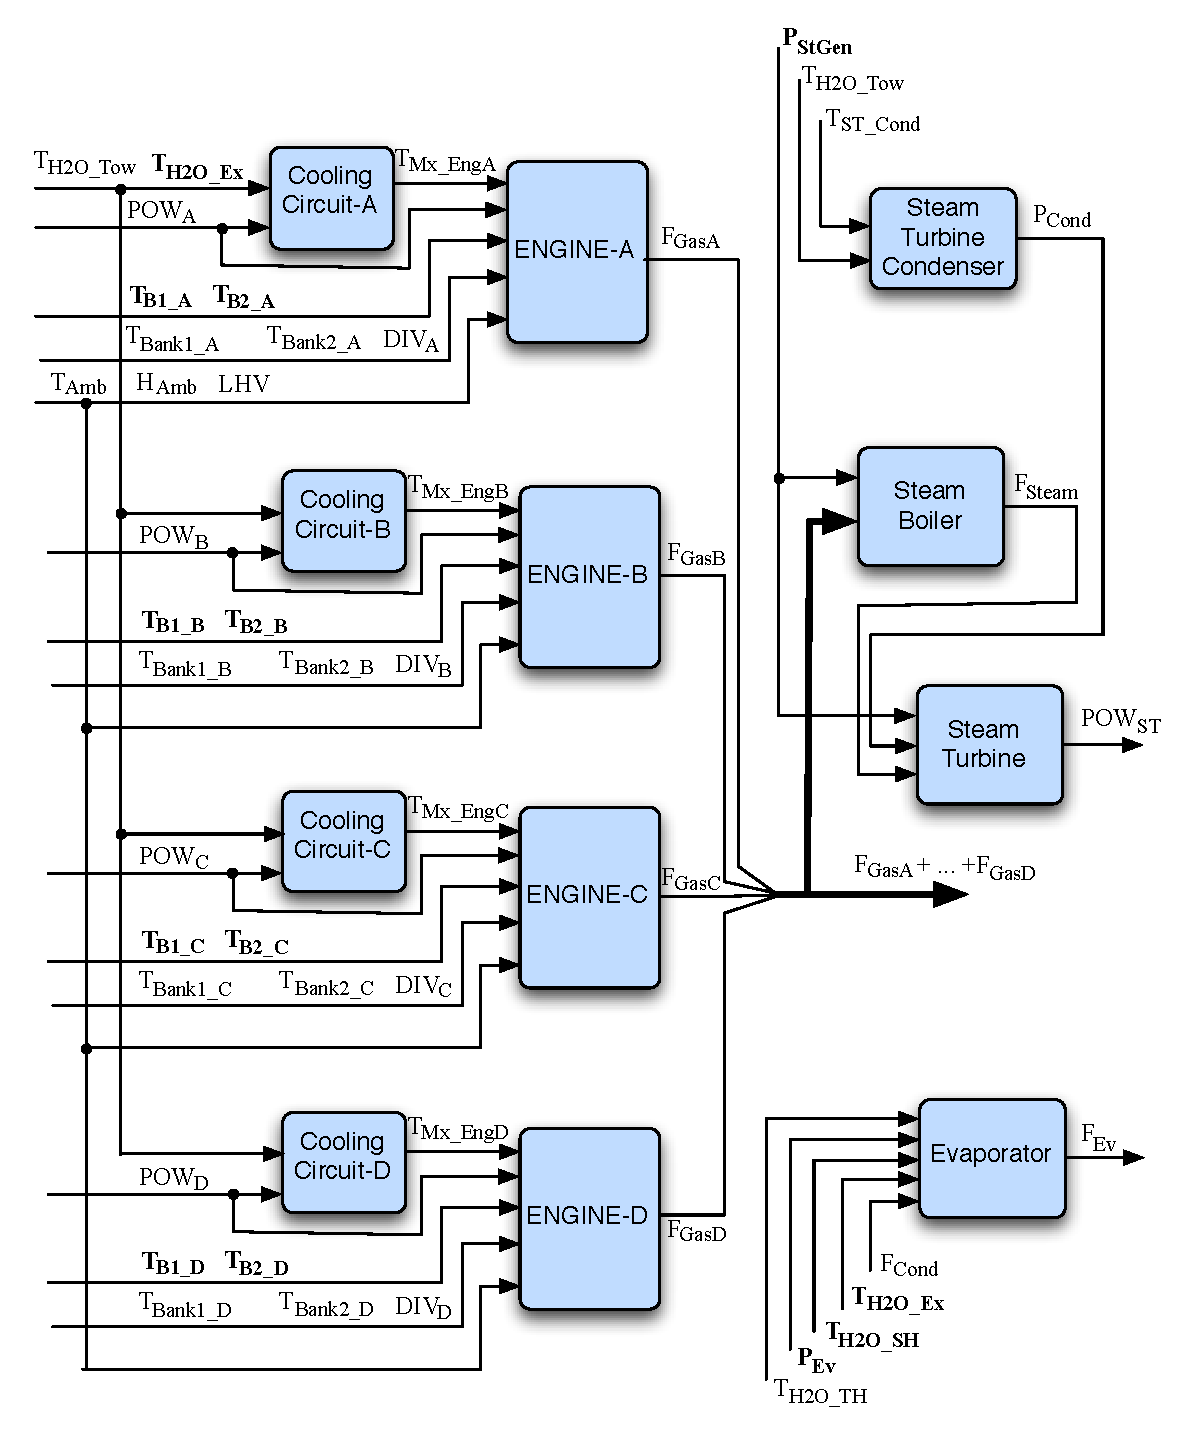
\includegraphics[width=1\textwidth]{NNs.pdf}
\caption{Modeling of the CHP Plant by means of interconnected NNs. Each block represents a NN.}
\label{fignns}
\end{figure}


The result of the modeling is presented in Table \ref{tbl:mse} where the Mean Squared Error (MSE) between the desired and actual output, for both the training and the testing phase, is shown. We can see that, in all the cases, the obtained  errors are very small, even in the testing case, where the NNs deal with unseen data. These results validate the modeling performance of the trained NNs. 

\begin{table}[!t]
\label{tbl:mse}
  \centering
\caption{MSE for training and testing samples for each Neural Network.}
\label{MSE} %\centering
\begin{tabular}{lrrrr} \toprule
 & Structure* & Iterations & Train Error & Test Error \\ \midrule
Cooling Engine A & 3/6/1 & \num{6000} & \SI{0.21}{\percent} & \SI{0.23}{\percent} \\
Cooling Engine B & 3/6/1 & \num{6000} & \SI{0.28}{\percent} & \SI{0.26}{\percent} \\
Cooling Engine C & 3/6/1 & \num{6000} & \SI{0.10}{\percent} & \SI{0.13}{\percent} \\
Cooling Engine D & 3/6/1 & \num{6000} & \SI{0.49}{\percent} & \SI{0.33}{\percent} \\
 Engine A & 10/20/1 & \num{20000} & \SI{0.39}{\percent} & \SI{0.42}{\percent} \\
 Engine B & 10/20/1 & \num{20000} & \SI{0.41}{\percent} & \SI{0.41}{\percent} \\
 Engine C & 10/20/1 & \num{20000} & \SI{0.38}{\percent} & \SI{0.42}{\percent} \\
 Engine D & 10/20/1 & \num{20000} & \SI{0.38}{\percent} & \SI{0.37}{\percent} \\
 Recovery Boiler & 2/4/1 & \num{4000} & \SI{0.61}{\percent} & \SI{0.63}{\percent} \\
 Steam Condenser & 2/4/1 & \num{4000} & \SI{1.01}{\percent} & \SI{0.96}{\percent} \\
 Steam Turbine & 3/6/1 & \num{6000} & \SI{0.67}{\percent} & \SI{0.70}{\percent} \\
 Slurry Process & 5/10/1 & \num{10000} & \SI{2.35}{\percent} & \SI{2.52}{\percent} \\
 \bottomrule
\end{tabular}
\vspace{-0.3cm}

\end{table}


To better appreciate the predicting ability of the NNs, we have also plotted, in Figures \ref{TcoolA} to  \ref{Pturbine}, the predicted data and the real data, for the variables $T_{Mixt\_EngA}$, $F_{GasA}$, $P_{Cond}$, $F_{Steam}$ and $POW_{ST}$. In particular, we have plotted the testing points of one week, corresponding to the Cooling Circuit of one Engine and to the Steam Turbine Condenser. We can observe how the  real and predicted curves are quite similar in both examples, confirming thus that the NNs are able to learn properly the dynamics of the plant. 

\begin{figure}
\centering
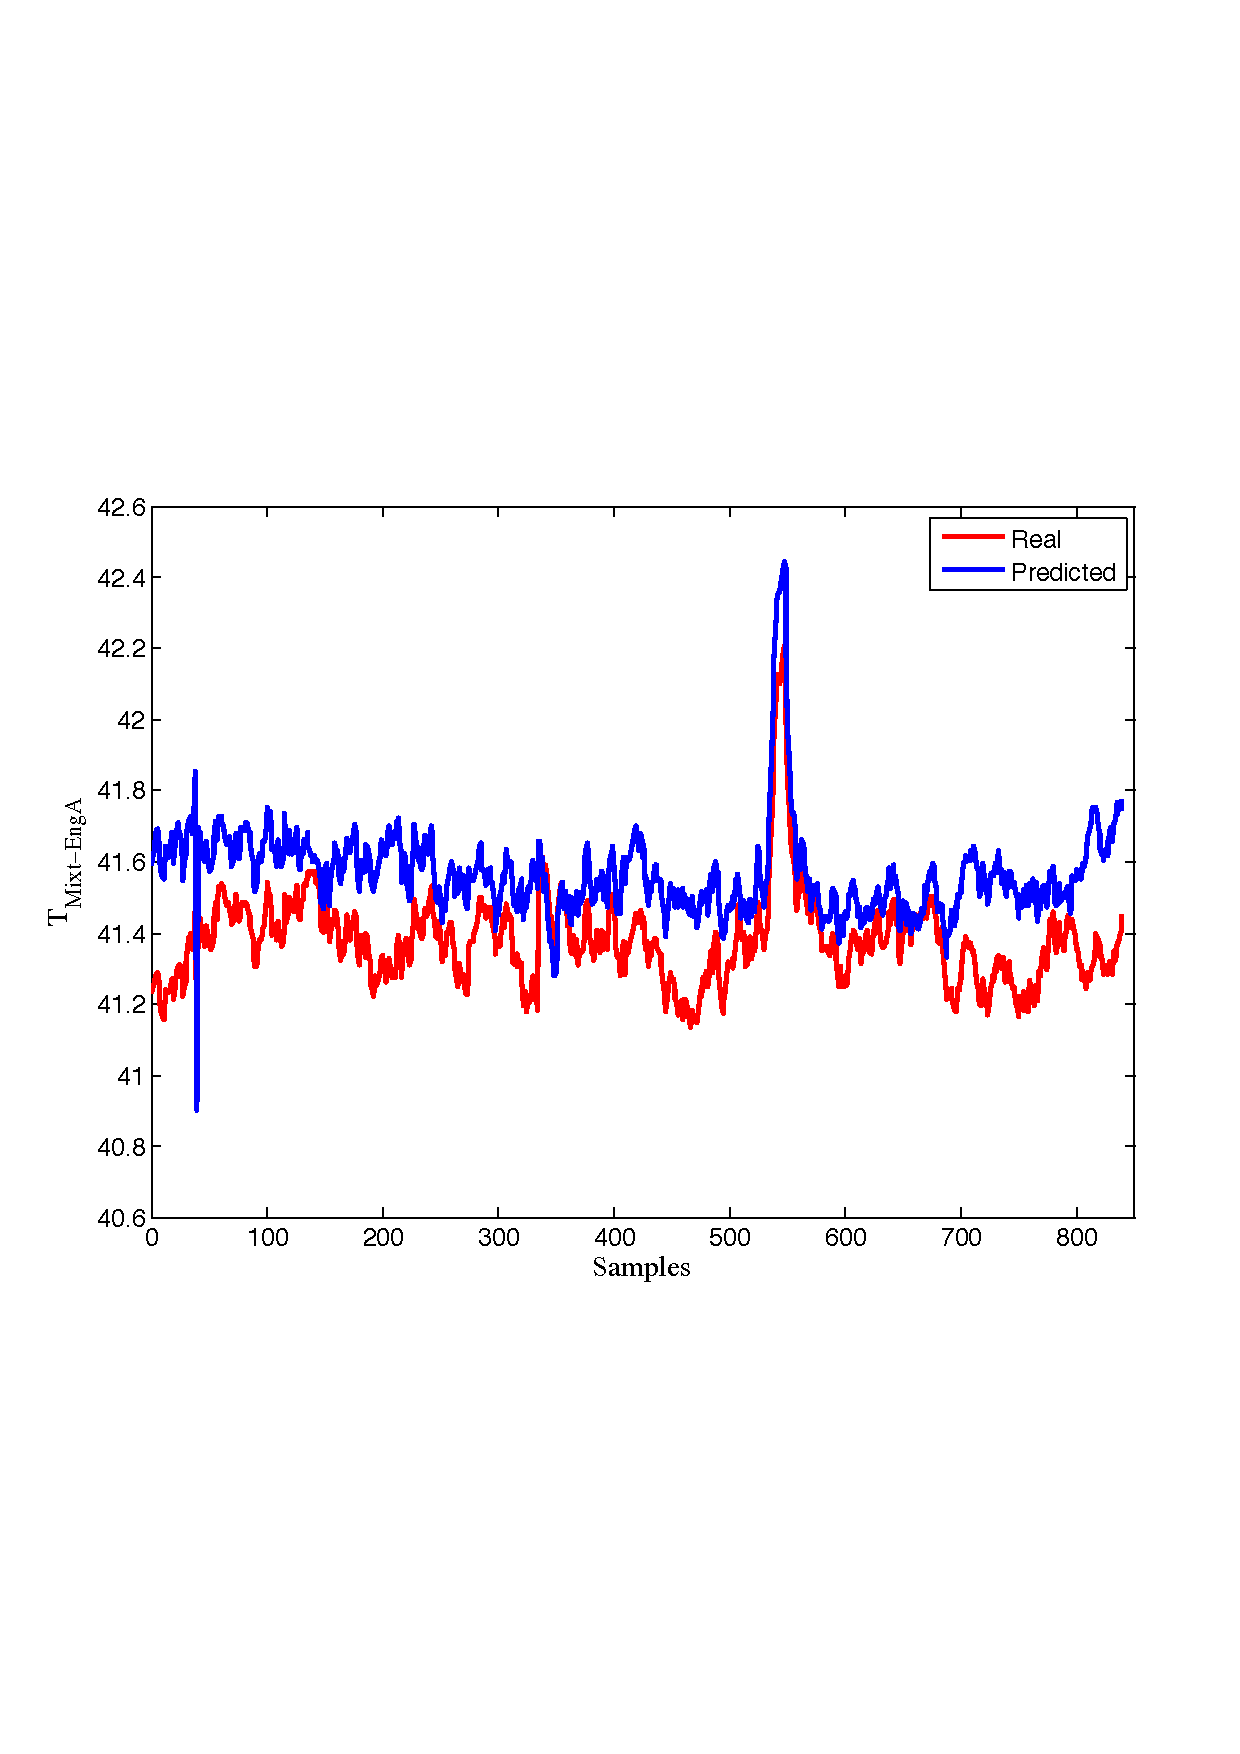
\includegraphics[width=0.7\textwidth]{nna0bis.pdf}
\caption{Real data and NN predicted data for the Cooling Circuit Temperature of Engine A ($T_{Mixt\_EngA}$) during a period of a week.}
\label{TcoolA}
\end{figure}

\begin{figure}
\centering
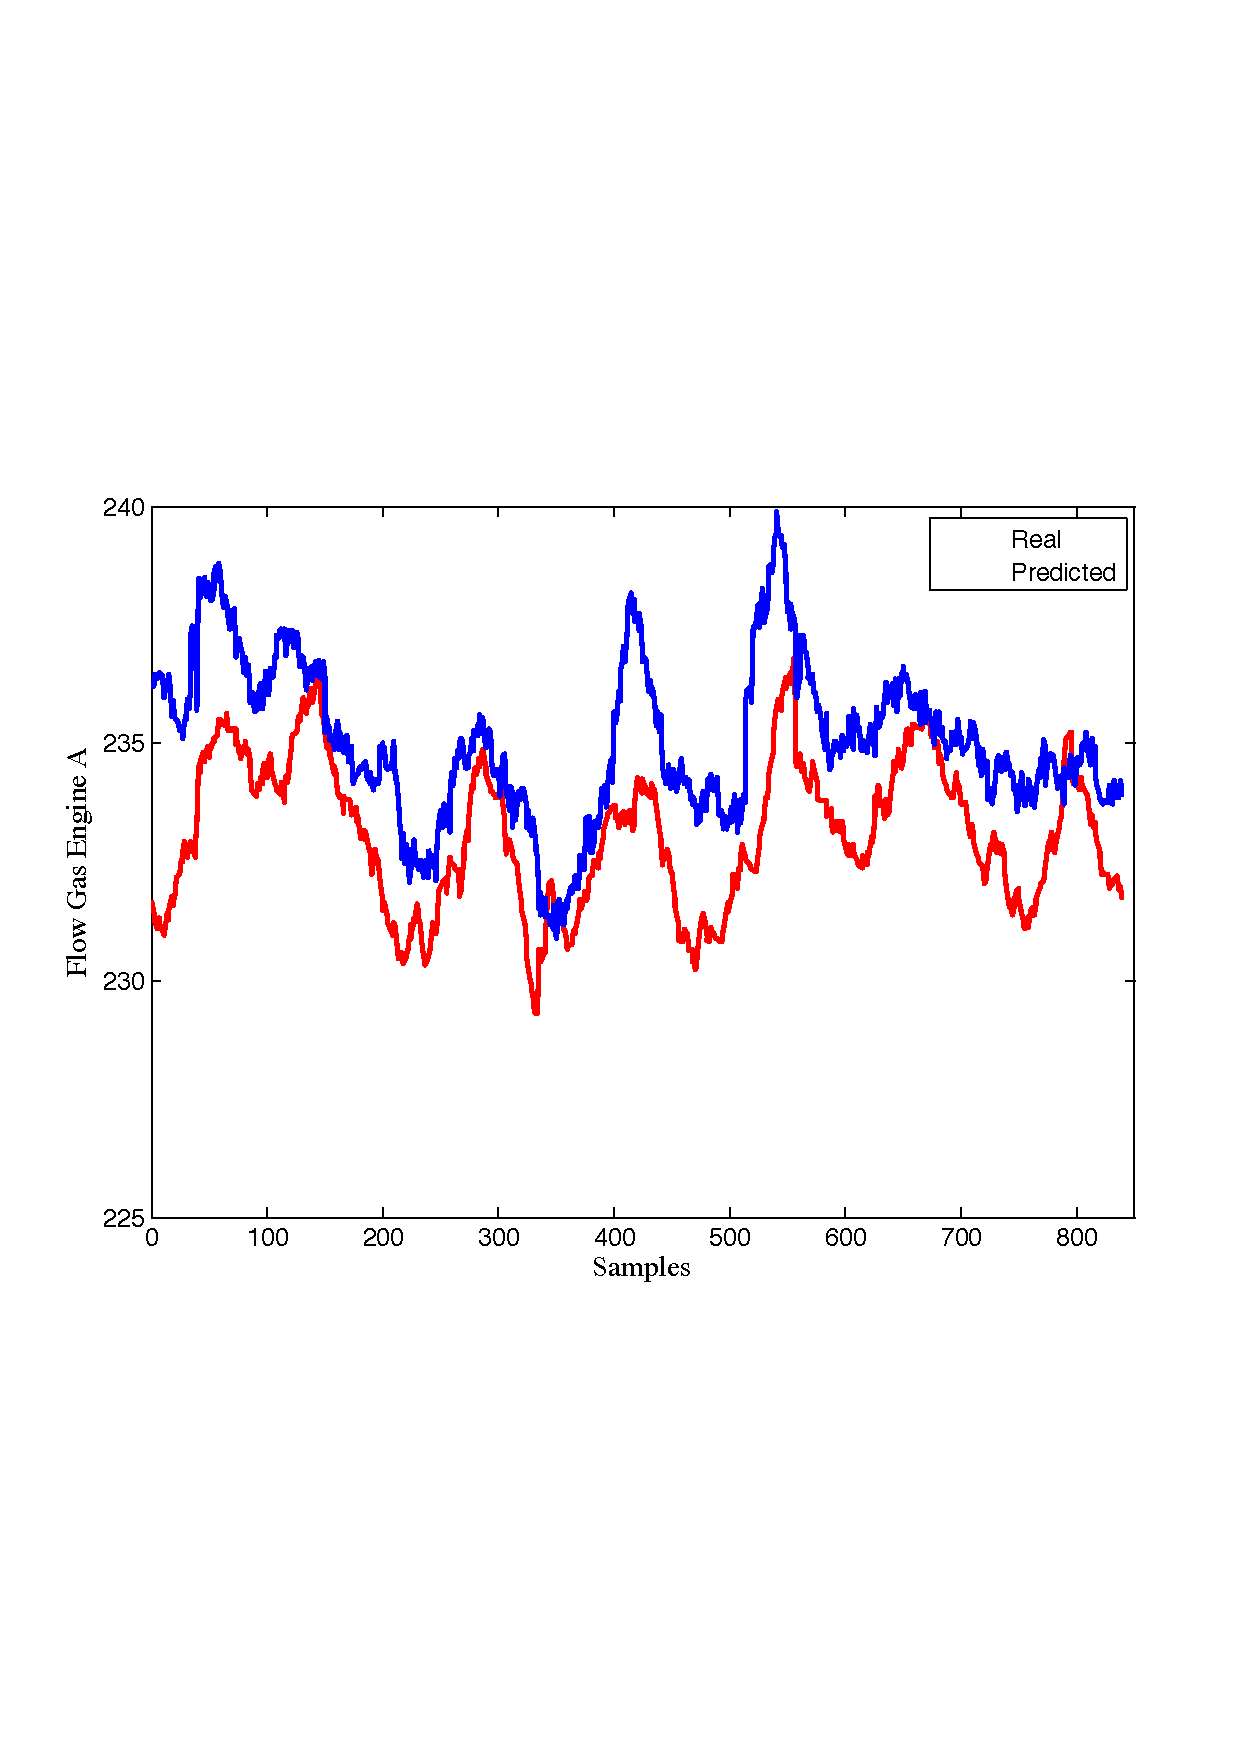
\includegraphics[width=0.7\textwidth]{nna1bis.pdf}
\caption{Real data and NN predicted data for the Natural Gas Flow  of Engine A ($F_{GasA}$). during a period of a week}
\label{FengineA}
\end{figure}

\begin{figure}
\centering
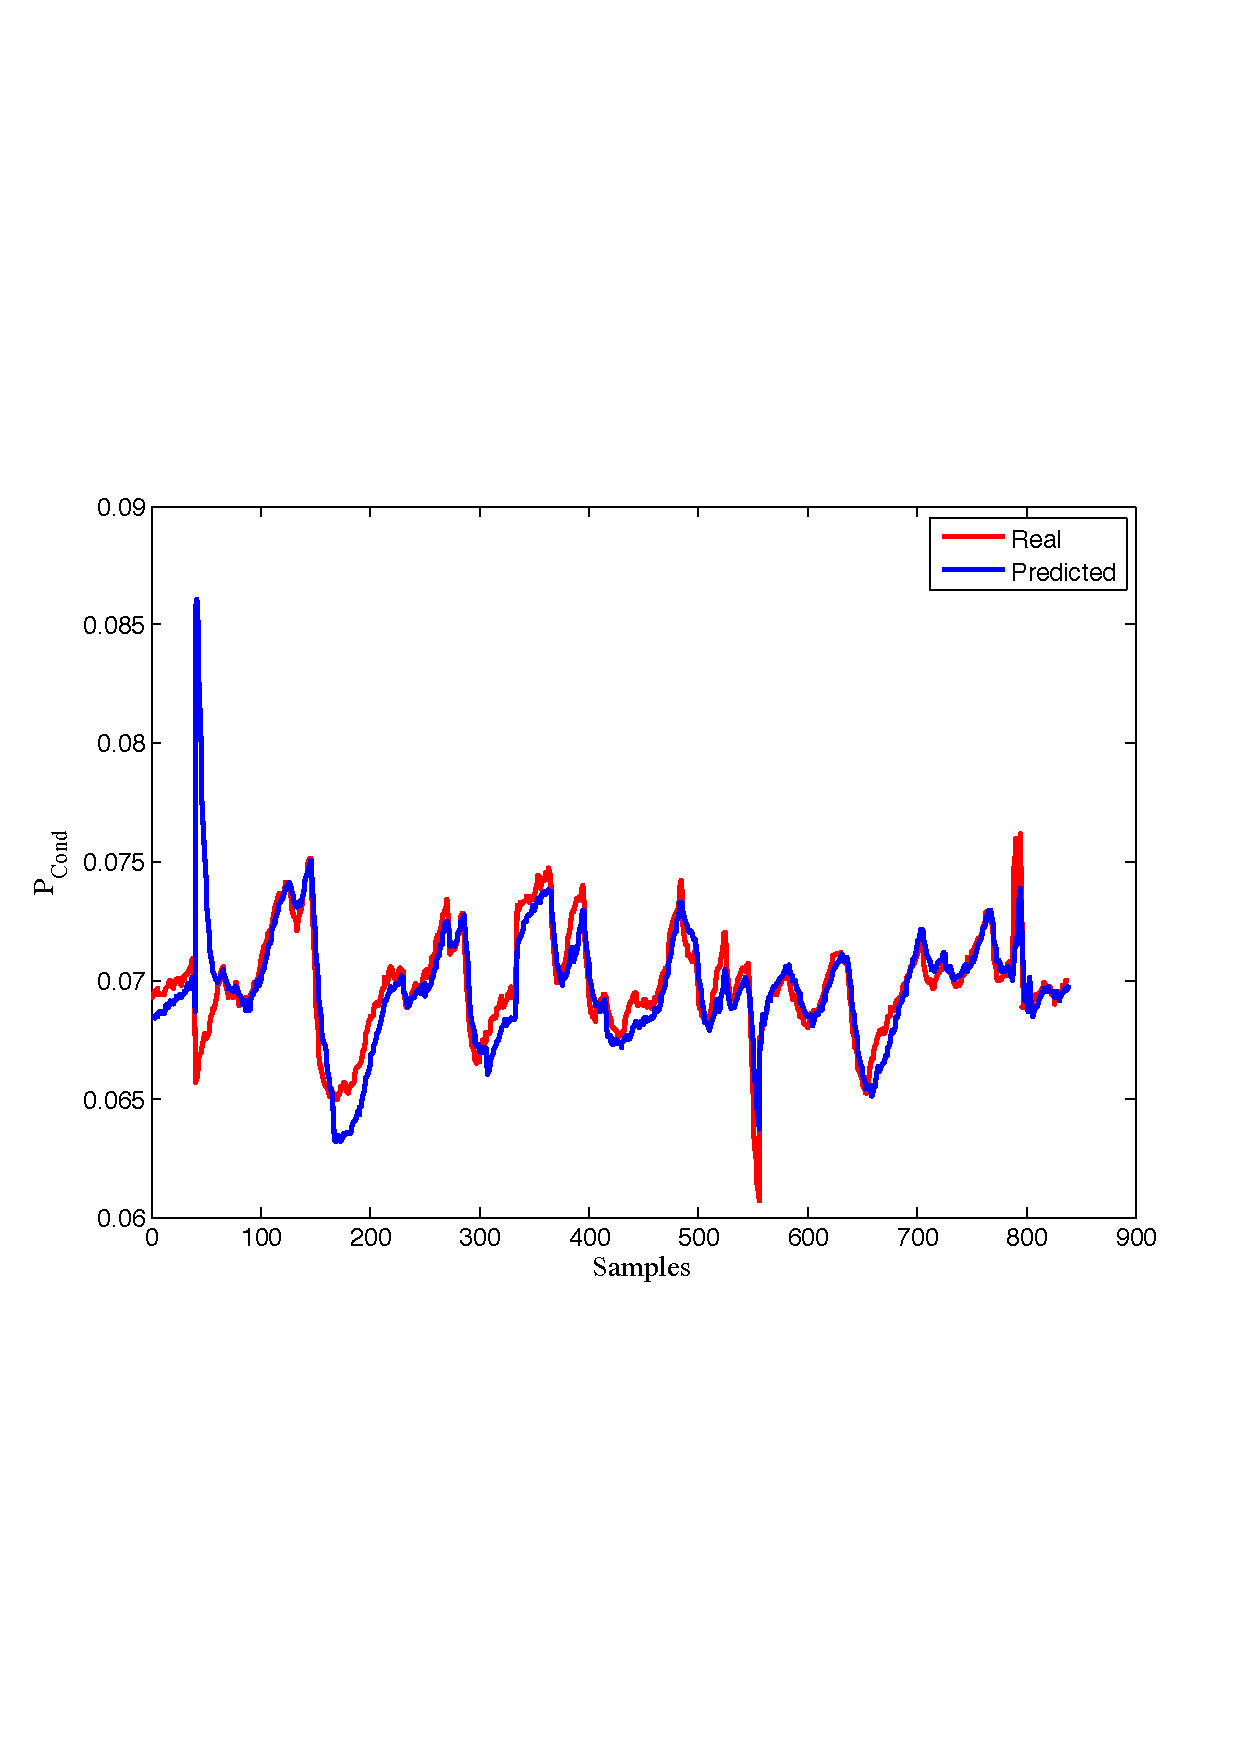
\includegraphics[width=0.7\textwidth]{nne0bis.pdf}
\caption{Real data and NN predicted data for the Steam Pressure of the Condenser  ($P_{Cond}$) during a period of a week.}
\label{Pcond}
\end{figure}

\begin{figure}
\centering
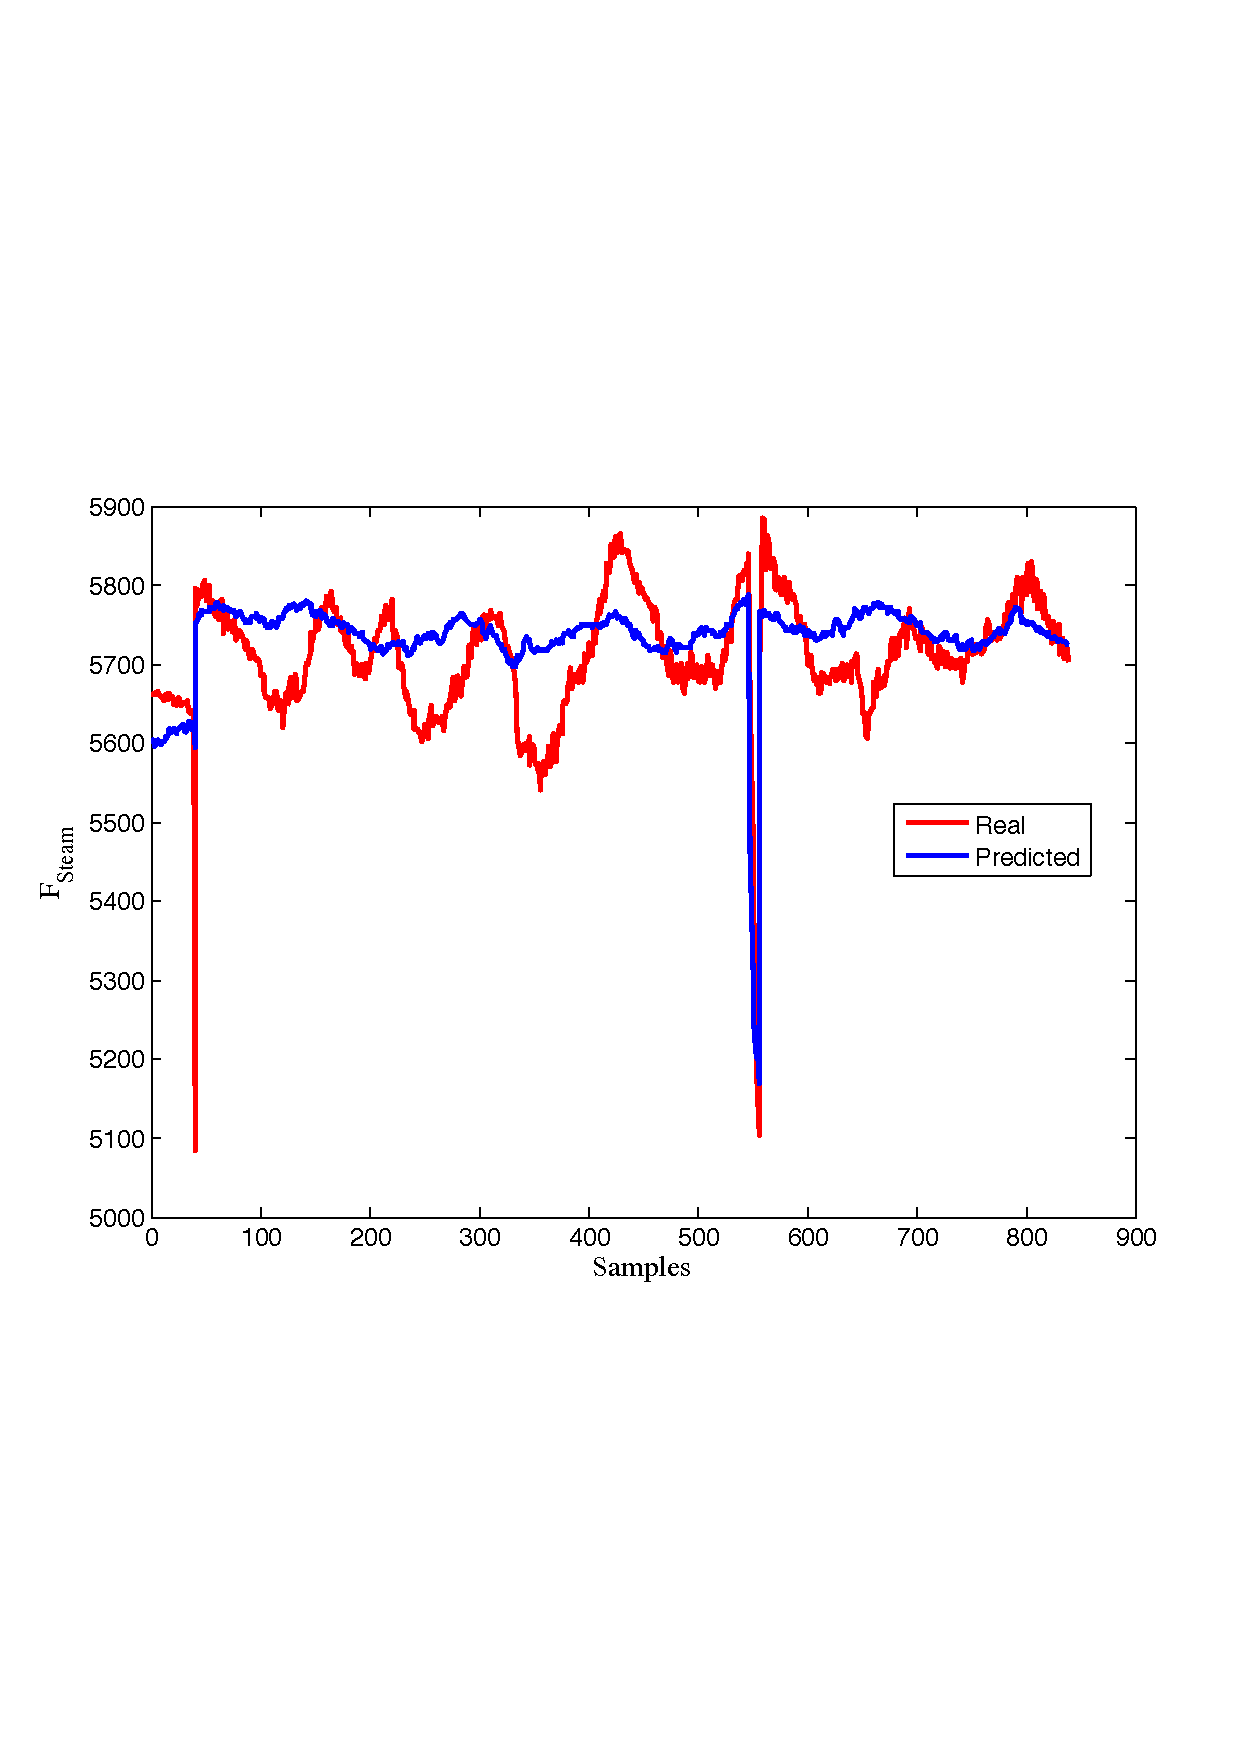
\includegraphics[width=0.7\textwidth]{nne1bis.pdf}
\caption{Real data and NN predicted data for the Steam Flow in the Boiler($F_{Steam}$) during a period of a week.}
\label{Fboiler}
\end{figure}

\begin{figure}
\centering
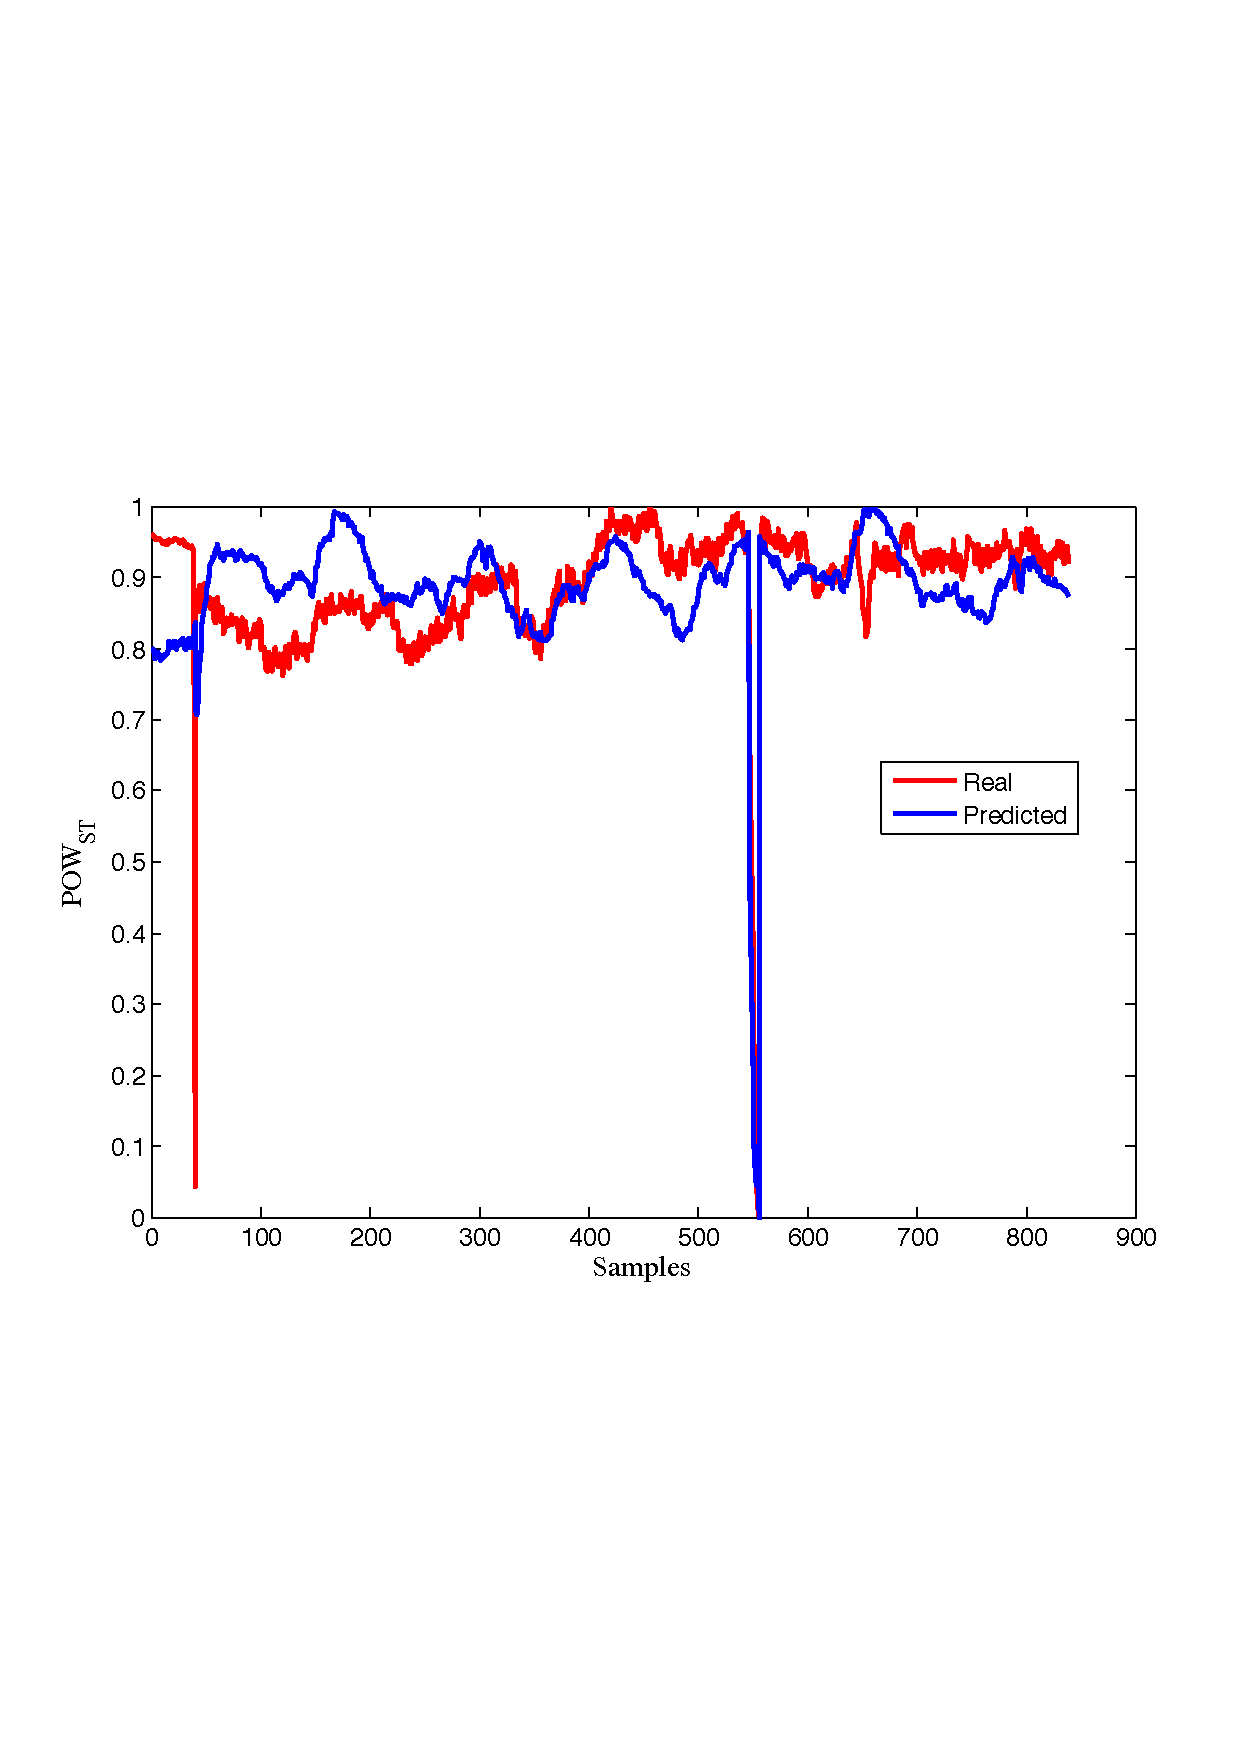
\includegraphics[width=0.7\textwidth]{nne2bis.pdf}
\caption{Real data and NN predicted data for the Power generated in the Turbine ($POW_{ST}$) during a period of a week.}
\label{Pturbine}
\end{figure}


%\begin{figure}
%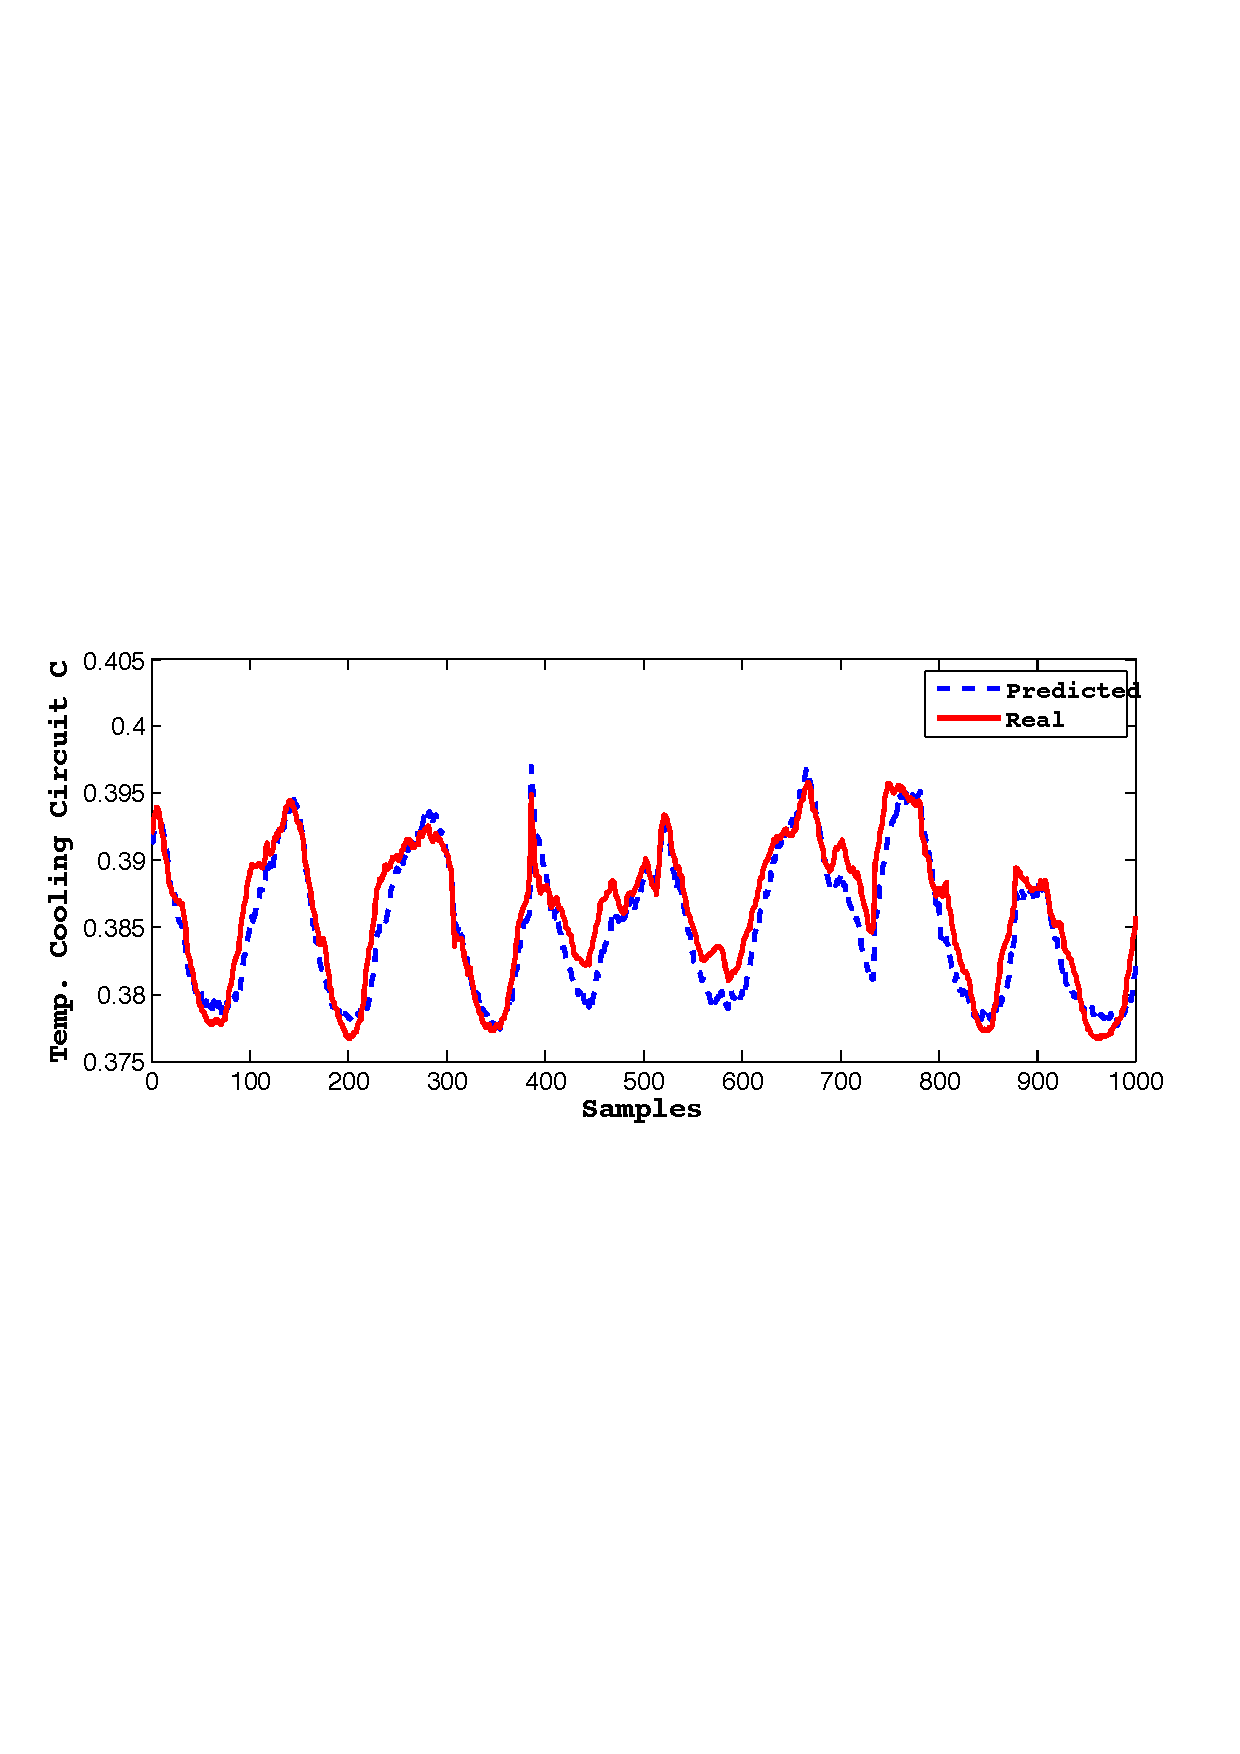
\includegraphics[width=1\textwidth]{TT3219.pdf}
%\caption{Real data and NN predicted data for the Cooling Circuit Temperature of Engine C ($T_{Mixt\_EngC}$) during a period of a week}
%\label{tcool}
%\end{figure}


%\begin{figure}
%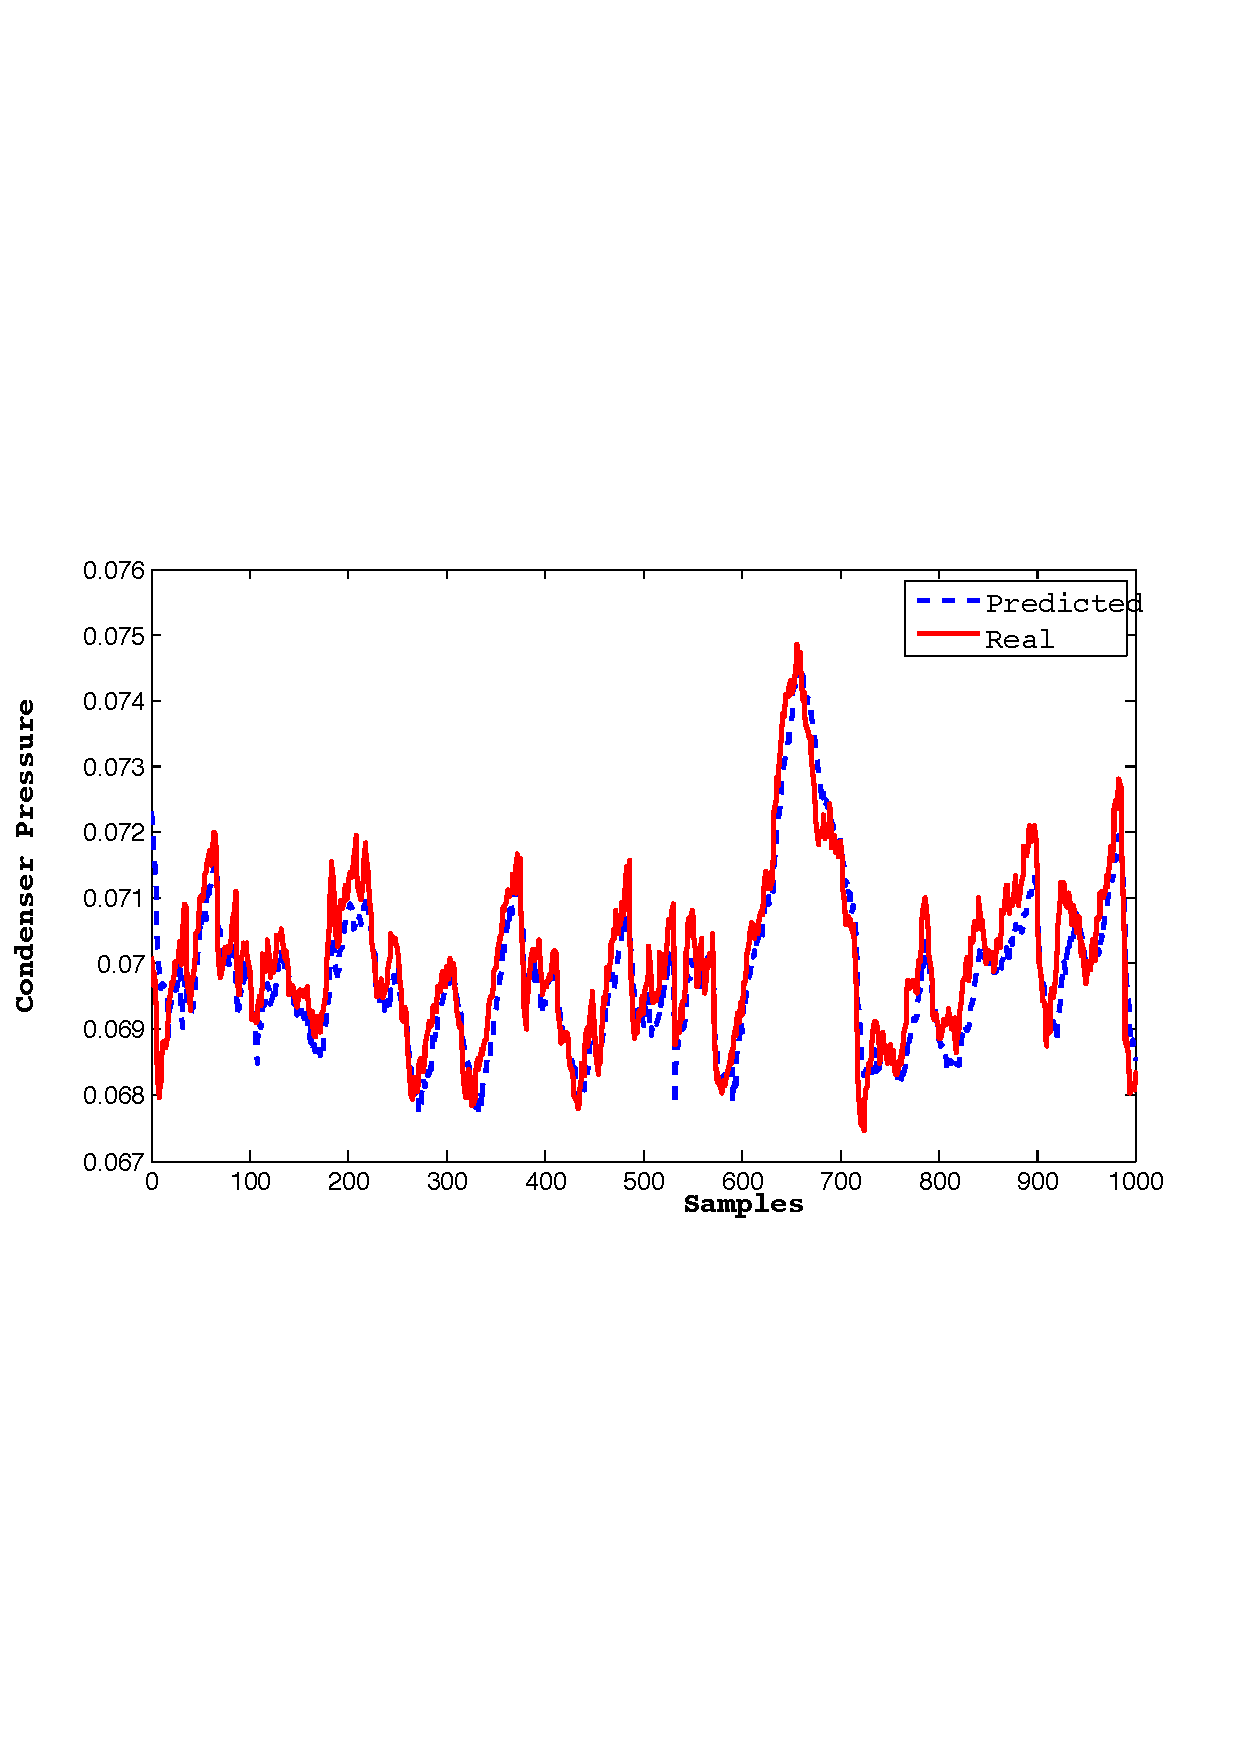
\includegraphics[width=1\textwidth]{ConPres.pdf}
%\caption{Real data and NN predicted data for the Condenser Pressure ($P_{Con}$) during a period of a week}
%\label{pcool}
%\end{figure}